\documentclass[times,specification,annotation]{itmo-student-thesis}

%% Опции пакета:
%% - specification - если есть, генерируется задание, иначе не генерируется
%% - annotation - если есть, генерируется аннотация, иначе не генерируется
%% - times - делает все шрифтом Times New Roman, собирается с помощью xelatex
%% - pscyr - делает все шрифтом Times New Roman, требует пакета pscyr.

%% Делает запятую в формулах более интеллектуальной, например:
%% $1,5x$ будет читаться как полтора икса, а не один запятая пять иксов.
%% Однако если написать $1, 5x$, то все будет как прежде.
\usepackage{icomma}

%% Один из пакетов, позволяющий делать таблицы на всю ширину текста.
\usepackage{tabularx}

\usepackage{tikz}

\usetikzlibrary{arrows.meta, fit, automata, positioning}

\usepackage{mathtools}

\usepackage{makecell}

\graphicspath{ {./images/} }

%% Указываем файл с библиографией.
\addbibresource{bachelor-thesis.bib}

\begin{document}

\studygroup{M3439}
\title{Обучение метрики похожести сообществ с помощью выделения
векторного представления}
\author{Зернов Глеб Сергеевич}{Зернов Г.С.}
\supervisor{Сметанников Иван Борисович}{Сметанников И.Б.}{к.техн.н.}{ассистент, факультет информационных технологий и программирования, Университет ИТМО}
\publishyear{2019}
%% Дата выдачи задания. Можно не указывать, тогда надо будет заполнить от руки.
\startdate{18}{декабря}{2018}
%% Срок сдачи студентом работы. Можно не указывать, тогда надо будет заполнить от руки.
\finishdate{6}{мая}{2019}
%% Дата защиты. Можно не указывать, тогда надо будет заполнить от руки.
\defencedate{}{}{2019}

\addconsultant{Попов А.Л.}{магистр}

\secretary{Павлова О.Н.}

%% Задание
%%% Техническое задание и исходные данные к работе
\technicalspec{Разработать модель, которая позволит представить сообщества социальной сети в
виде векторов. Модель необходимо обучить и протестировать на анонимных неразмеченных
сессионных данных из социальной сети «Вконтакте». Необходимо проанализировать
результаты и сравнить предлагаемое решение с альтернативными методами.}

%%% Содержание выпускной квалификационной работы (перечень подлежащих разработке вопросов)
\plannedcontents{
\begin{enumerate}
\item[1.] Описание предметной области. Обзор существующих подходов.
\item[2.] Описание моделей векторного представления сообществ
\item[3.] Анализ результатов, сравнение с существующими решениями.
\end{enumerate}}

%%% Исходные материалы и пособия 
\plannedsources{\begin{enumerate}
    \item T. Mikolov [и др.] Distributed representations of words and phrases and their compositionality // Advances in neural information processing systems. — 2013. — С. 3111–3119.
    \item Grbovic M., Cheng H. Real-time Personalization using Embeddings for Search Ranking at Airbnb // Proceedings of the 24th ACM SIGKDD International Conference on Knowledge Discovery and Data Mining.  — 2018.  —
С. 311–320.
    \item Vasile F., Smirnova E., Conneau A. Meta-Prod2Vec: Product Embeddings Using Side-Information for Recommendation // Proceedings of the 10th ACM Conference on Recommender Systems. — ACM, 2016. — C. 225–232.
\end{enumerate}}

%%% Цель исследования
\researchaim{Получение моделей представления сообществ социальной сети в виде векторов.}

%%% Задачи, решаемые в ВКР
\researchtargets{\begin{enumerate}
    \item Обзор существующих подходов.
    \item Разработка моделей выделения векторного представления сообществ по сессионным анонимным неразмеченным
данным. 
    \item Анализ полученных результатов.
\end{enumerate}}

%%% Использование современных пакетов компьютерных программ и технологий
\addadvancedsoftware{Язык программирования \texttt{Python}}{
    \ref{sec:algo-subs} - \ref{sec:visual}
}
\addadvancedsoftware{Программное средство \texttt{Jupyter Notebook}}{\ref{sec:algo-subs} - \ref{sec:visual}}
\addadvancedsoftware{Библиотека \texttt{Pytorch}}{\ref{sec:algo-subs} - \ref{sec:algo-combined}}
\addadvancedsoftware{Библиотека \texttt{Sklearn}}{\ref{sec:class}, \ref{sec:geo}, \ref{sec:visual}}
\addadvancedsoftware{Библиотека \texttt{Matplotlib}}{\ref{sec:visual}}
\addadvancedsoftware{Библиотека \texttt{Spark} и язык программирования \texttt{Skala}}{\ref{sec:class}}

%%% Краткая характеристика полученных результатов 
\researchsummary{Исследованы существующие решения данной задачи. Получены модели, позволяющие представить сообщества социальной сети в виде векторов. Проведено сравнение предложенного решения с существующими путем решения дополнительных задач классификации с использованием результатов работы
моделей в качестве входных данных, а так же задачи предсказания следующего действия пользователя. Произведена иллюстрация векторов, полученных в результаты работы обучения одной из предложенных моделей.}

%%% Гранты, полученные при выполнении работы 
\researchfunding{При выполнении работы грантов получено не было.}

%%% Наличие публикаций и выступлений на конференциях по теме выпускной работы
\researchpublications{Нет}

%% Эта команда генерирует титульный лист и аннотацию.
\maketitle{Бакалавр}

%% Оглавление
\tableofcontents

%% Макрос для введения. Совместим со старым стилевиком.
\startprefacepage

\startrelatedwork

Социальные сети стали неотъемлемой частью современной жизни. Большая часть самых популярных сайтов являются социальными сетями \footnote{https://www.alexa.com/topsites}, а число их пользователей стремительно растет каждый год. Около 80\% всех пользователей сети Интернет --- активные пользователи социальных сетей. \footnote{https://datareportal.com/reports/digital-2019-global-digital-overview}  

Особенностью социальных сетей является огромное число контента, производимого пользователями. Текст, видео, фото, взаимодействия пользователей между собой --- все это создает больше обьемы информации. Анализ этой информации является сложной, но необходимой для развития платформы, задачей.

Например, для улучшения пользовательского опыта социальные сети используют множество алгоритмов машинного обучения. Персонализированная реклама и рекомендации контента, предложения добавить пользователя в список друзей, анализ пользовательской активности и многое другое. Однако, для обучения моделей необходимы данные об объектах сети. Проблема заключается в том, что данных о сущностях социальной сети очень много и использование всей информации не только является сложной инженерной задачей, но и требует огромных трат ресурсов.   

Альтернативным способом представления сущностей выступают модели машинного обучения, позволяющие представить объекты в сжатом виде в качестве векторов, которые описывают объект и его свойства.

Алгоритмы векторного представления объектов получили широкое распространение и используются в различных областях, в том числе и в социальных сетях. Например, социальная сеть Pinterest\footnote{https://www.pinterest.com} \cite{Liu2017} использует модель векторизации объектов социальной сети (Pin'ов), сервис YouTube\footnote{https://youtube.com} использует алгоритмы векторного представления для рекомендации видео\cite{Covington2016} 

В данной работе рассматриваются алгоритмы построения такого представления для сообществ социальной сети. В первой главе описывается постановка задачи и производится обзор существующих способов решения задачи. Во второй главе описывается алгоритм обучения модели, которая позволяет строить векторные представления сообществ по сессионным данным пользовательской активности. Рассматриваются три вариации модели: базовая, позволяющая работать с позитивными и негативными редкими откликами пользователя, альтернативная, работающая со слабыми и частыми сигналами и комбинированная, учитывающая оба типа пользовательской активности. В заключительной главе проводятся эксперименты по сравнению предложенных моделей с альтернативными вариантами, а также сравниваются вариации конечной модели между собой путем решения дополнительных задач. 

%% Начало содержательной части.
\chapter{Описание предметной области}

<<Вконтакте>>\footnote{https://vk.com} --- одна из крупнейших социальных сетей СНГ и самая
популярная соц. сеть в России. <<Вконтакте>> на ряду с многими другими
социальными сетями предоставлять возможность пользователям создавать объединения по интересам,
называемые сообществами. Пользователи имеют возможность подписаться на
интересуемое их сообщество для более удобного взаимодействия с информацией
сообщества, а также отписаться от него. Сообщества могут добавлять на свою
страницу записи (текст, картинки, видео и т. д.), которые пользователи могут
помечать как понравившиеся (<<лайки>>), комментировать и прочее.

Существенной сложностью работы с сообществами является число сообществ (миллионы), каждое из которых может состоять из миллионов пользователей.  

Таким образом, полная информация о сообществе --- это огромный массив
данных, предоставляя который полностью некоторой модели машинного обучения,
с одной стороны существенно увеличивается размер необходимого объeма памяти для хранения этой информации, а с другой --- замедляется работа самого алгоритма, что потенциально делает алгоритм бесполезным для применения на практике.

Выходом из этой ситуации является некоторое более eмкое представление сообщества без потери интересующей информации в виде вектора.

Такие векторы используются в большом спектре прикладных задач в качестве входных данных моделей машинного обучения. Область применения включает, но не ограничивается, задачами классификации сообществ по некоторым признакам, что позволяет получить более подробное представление о природе сообщества, предсказанием следующего действия пользователя, для рекомендаций сообществ пользователю, кластеризации --- сообщества в одном кластере могут быть рекомендованы пользователю, который заинтересован другими сообществами этого кластера, либо для рекламы сообществ кластера пользователям, состоящим в других сообществах этого кластера. 

Задача, решаемая в моей работе, --- получить модели для выделения универсального векторного представление сообществ небольшой размерности. Полученное векторное представление обязано сохранять семантический смысл сообществ, т.е. два сообщества, которые находятся близко в конечном векторном пространстве, должны быть похожи между собой семантически. 

\section{Основные определения}\label{sec:def}

\textbf{Машинное обучение} (\textit{англ. machine learning}) --- класс алгоритмов и статистических моделей. Модели, построенные алгоритмами машинного обучения, способны решать некоторую задачу без явных программных указаний, основываясь на предоставленных модели данных.   

\textbf{Обучение с учителем} (\textit{англ. supervised learning}) --- раздел машинного обучения, в котором обучение моделей происходит с помощью размеченного набора данных, т.е. для каждого входного значения сопоставляется правильный <<ответ>> --- выходное значение. Такие модели анализируют связи между входными и выходными значениями среди всего набора данных и пытаются предсказать ответы по входным значениям. 

\textbf{Обучение без учителя} (\textit{англ. Unsupervised learning}) --- раздел машинного обучения, в котором обучение моделей происходит без явных выходных сигналов. Такие модели анализируют статистические связи между объектами и пытаются выделить некоторые обобщающие признаки объектов.

\textbf{Унитарный код} (\textit{англ. one-hot}) --- способ векторного представления объектов. Для такого кодирования создается список всех объектов, затем объекты нумеруются, и в конце кодируются следующим образом: создается вектор размерности $N$ ($N$ --- число уникальных объектов, длина списка), полностью состоящий из нулей, за исключением позиции $i$, на которой стоит единица. В таком случае $i$ --- номер кодируемого объекта в списке. 

\textbf{Косинусное сходство} (\textit{англ. cosin similarity}) --- метрика сходства двух векторов, измеряющая косинус угла между ними и задается формулой через скалярное произведение векторов:
 \begin{align*}
 cosin\_similarity(x, y) = \frac{x \cdot y}{\lVert x \rVert \lVert y \rVert} 
 \end{align*}
 
\textbf{Задача классификации} --- разделение объектов на классы является распространненой задачей, которая решается методами машинного обучения. Существует множество алгоритмов машинного обучения для решения этой задачи.

\textbf{Метод опорных векторов} \cite{cortest1995} (\textit{англ. support vector machine})  --- метод машинного обучения для решения ряда задач, в том числе задачи классификации. Задачей таких моделей является нахождение оптимальной гиперплоскости (с максимальным расстоянием до представителей) в пространстве, разделяющей представителей разных классов. 

\textbf{Дерево решений} \cite{quinlan1986induction} (\textit{англ. decision tree}) --- дерево, листьями которого являются значения класса объекта, а в вершинах записаны условия перехода по ребрам. Таким образом, в процессе обучения изменяются коэффициенты функций условий переходов.   

\textbf{Бустинг} (\textit{англ. boosting}) --- методика машинного обучения, позволяющая объединять несколько слабых классификаторов (например, деревья решений) в один сильный. Существует множество методов бустинга, к примеру градиентный бустинг\cite{friedman2002stochastic}, использующий градиентный спуск для уменьшения функции потери, задаваемой ошибкой классификатора, адаптивный бустинг (более известный как Agaptive Boosting или AdaBoost)\cite{freund1997decision}, создающий веса для каждого классификатора, усиливая, таким образом, влияние лучших классификаторов.  

\textbf{F-мера} (\textit{англ. F-measure или $F_1 score$}) --- метрика оценки качества модели. Задается формулами
 \begin{align*}
F_1 = 2 \frac{precision \cdot recall}{precision + recall}
\end{align*}
 \begin{align*}
precision = \frac{true_positive}{true_positive + false_positive}
\end{align*}
 \begin{align*}
recall = \frac{true_positive}{true_positive + false_negative}
\end{align*}
Где $true_positive$ --- число истинно позитивных результатов, $false_positive$ --- число ложно позитивных результатов, $false_negative$ --- число ложно негативных результатов.

\textbf{t-SNE} (\textit{T-distributed Stochastic Neighbor Embedding})\cite{maaten2008visualizing} --- алгоритм машинного обучения, позволяющий понизить размерность векторного пространства, при обучении модель пытается приблизить вероятность похожести двух объектов в конечном пространстве к той же вероятности в изначальном пространстве. Таким образом, конечное пространство (чаще всего двухмерное) позволяет визуализировать исходное многомерное пространство с учетом похожести объектов. 

\textbf{Метод k-средних} (\textit{англ. k-means})\cite{lloyd1982least} --- алгоритм кластеризации, выделяющий $k$ кластеров и минимизирующий функцию потерь (среднеквадратичное отклонение) от представителей кластера до центра.  

\section{Постановка задачи}\label{sec:intro}

Поставленная задача формализуется следующим образом: для заданного множества $C$ сообществ, пользователей $N$ и сессий пользовательской активности $A_n$, $n \in N$ найти представление $v_{c} \in \mathbb{R}^d$ размерности $d$ для каждого сообщества $c \in C$ так, что семантически похожие сообщества находятся близко друг к другу в конечном векторном пространстве. 

Данная задача решается для 3 случаев представления сессий $A_n$
 
В первом случае сессия состоит из множества событий двух типов:
 \begin{align}
A_n = (S_n, U_n) 
\label{eq-subs}
\end{align}
Где события $S_n$ --- список последовательных $K$ уникальных подписок на сообщества пользователя $n$ за некоторый промежуток времени: $S_n = (c_{1}, c_{2}, \dots, c_{K}), \forall i \ne j : c_i \ne c_j$, а $U_n$ --- список последовательных $M$ уникальных отписок от сообществ пользователя $n$: $U_n = (c_{1},  c_{2}, \dots, c_{M}), \forall i \ne j : c_i \ne c_j$, $S_n \cap U_n = \varnothing$.

Во втором случае сессия задаeтся как множество $K$ (не обязательно уникальных) действий (<<лайков>>) пользователя $n$ записей сообществ:
 \begin{align}
A_n = (c_{1}, c_{2}, \dots, c_{K}) 
\label{eq-likes}
\end{align}
 
В третьем случае каждой сессии задаeтся тип $T_n$ пользовательских событий, представленных в ней $T_n = \{subs, likes\}$ --- подписки/отписки, либо лайки. В таком случае сессия задается в зависимости от типа:
\begin{equation}
    A_n =
    \begin{cases}
      (S_n, U_n), & \text{if}\ T_n=subs \\
      (c_{1}, c_{2}, \dots, c_{K}), & \text{if}\ T_n=likes
    \end{cases}  
    \label{eq-combined}
  \end{equation}
 И определяется формулой (\ref{eq-subs}) для первого типа, формулой (\ref{eq-likes}) для второго.

\section{Обзор существующих решений}

\subsection{Алгоритм факторизации матриц в рекомендательных системах.}\label{sec:als}

Персонализация пользовательского контента является одной из основополагающих частей систем, предоставляющих такой контент конечным пользователям. Лидеры интернет-торговли или интернет-услуг особенно заинтересованы в таких алгоритмах, поскольку это позволяет увеличить пользовательский отклик.
В общем случае, рекомендательные системы разделяются на две категории по общему принципу работы.
  
Первой категорией является фильтрация контента (\textit{англ. content filtering})\cite{Lops2011}. Главная идея состоит в том, чтобы создать профиль для каждого пользователя или продукта с целью охарактеризовать сущность. Например, в качестве профиля фильма могут выступать жанр, актeры, кассовые сборы и т.д.

Альтернативный вариант, коллаборативная фильтрация (\textit{англ. collaborative filtering}), опирается на действия пользователей, сделанных в прошлом. Такие алгоритмы анализируют статистические связи между пользователями, продуктами, их взаимодействиями и дают рекомендации, основываясь на исторических данных.  Большим плюсом таких систем является независимость от домена, в котором они применяются.

Одним из самых распространeнных на данный момент времени алгоритмов в сфере рекомендательных систем является алгоритм факторизации матриц \cite{koren2009}, относящийся к группе алгоритмов коллаборативной фильтрации.

Модель матричной факторизации переносит пользователей и продукты в пространство признаков размерности $n$. Таким образом, продукт $p$ представим в виде вектора $a_{p} \in \mathbb{R}^n$ , а пользователь $u$ в виде вектора $b_{u} \in \mathbb{R}^n$. Для продукта каждый из элементов вектора отвечает за то, насколько каждый признак характерен для  этого продукта. В то время для пользователя элементы вектора показывают, насколько пользователю интерес признак.

Это позволяет задать оценку пользователя $u$ продукта $p$ в виде формулы
 \begin{align*}
r_{ui} = a_{i}^{T}b_{u}
\end{align*}
Таким образом, зная матрицу пользовательских оценок $R$, можно разложить ее на произведение матриц $A$ и $B$, отвечающих за векторное произведение продуктов и пользователей соответственно.
 \begin{align*}
R = A^TB
\end{align*}

В рамках задачи, поставленной формулой(\ref{eq-subs}), матрица оценок составляется следующим образом: для подписки пользователя $i$ на сообщество $j$ выставляется единица на эту позицию $R_{ij} = 1$, аналогично для отписки $R_{ij} = - 1$. В случае отсутствия действий пользователя для сообщества оценка будет равна нулю.

Адаптируя алгоритм ALS \cite{koren2009} для представления сессий формулы (\ref{eq-likes}), можно представить оценку пользователя сообществу, как число <<лайков>>, которые он поставил этому сообществу за сессию.

Для работы с комбинированными данными (формула \ref{eq-combined}) эти два подхода объединяются. Конечная матрица составляется следующим образом: если сессия имеет тип $subs$, данные представляются, так, как описано в первом варианте (для подписок), иначе, как во втором. Поскольку подписка более важное событие, чем лайк, вводится коэффициент для подписок $q$, на который будут умножаться события из сессий типа $subs$.   

\subsection{Обзор алгоритма LDA}\label{sec:lda}

Latent Dirichlet allocation (LDA) \cite{lda2003} --- вероятностная модель над корпусом документов. Базовая идея заключается в том, что документы представимы в виде набора тем, где каждая тема характеризуется распределением по словам. Данная модель позволяет выделять несколько тем для документа и рассчитывать вероятности отношения каждой из тем к документу.
В качестве продукта работы алгоритма LDA позволяет строить вероятностные распределения тем по документу, слов по темам и темам по словам.

Например, для такой модели будет верно, что слово <<кот>> имеет большую вероятность того, что оно относится к теме, интерпретируемую наблюдателем как <<животные>> (имеет большие вероятности для слов, обозначающих животных), чем к другим темам. 

Стоит отметить, что несмотря на тот факт, что модель LDA была впервые применена в области NLP, это не ограничивает использование алгоритма в других доменах. Так, в оригинальной статье \cite{lda2003} приводится пример использования для коллаборативного фильтрования. Кроме того, модель может быть использована для поиска групп в графах \cite{Henderson2009}, для обнаружения классов объектов на изображениях, представленных в трeхмерном виде (обучение без учителя) \cite{Endres2009} и прочее.

В рамках данной работы (для задач, определяемых формулами (\ref{eq-subs}) и (\ref{eq-likes})) алгоритм LDA применим следующим образом: сессии представляются в виде документов, где словами являются подписки (лайки во втором случае) на сообщества. Применив алгоритм на корпусе сессий, получается список тем, а также вероятность принадлежности сообщества к теме для всех сообществ. Так составляется вектор вероятностей для каждого сообщества, которым можно охарактеризовать любое сообщество из всего словаря. Можно интерпретировать такое представление сообществ как то, что похожие сообщества будут иметь похожие вероятностные распределения тем. 

Для задачи, задаваемой формулой (\ref{eq-combined}), аналогично пункту \ref{sec:als} задается коэффициент $q$, на который будут умножаться события-подписки в модели (т.е. число слов в документе) 
 
Важным является тот факт, что модель не будет учитывать сигналы отписок от сообщества, и это является недостатком применения данного алгоритма. 

\section{Модели естественного языка}\label{sec:nlp-intro}

Для множества алгоритмов обработки естественного языка (Natural Language Processing, NLP) некие специализированные цели алгоритма могут быть обобщены на задачу нахождения значений вероятностей для последовательностей слов.
Таким образом, развитие алгоритмов обработки естественного языка шло путeм выявления статистических свойств слов и нахождения зависимостей между ними.

Традиционно такие подходы представляли каждое слово в виде one-hot вектора, однако недостатком такого представления является наложение ограничений на практическое применение алгоритмов, в связи с большой размерностью объектов и разряженности данных, приводящих к ощутимой потери производительности.

Исследователями были предложены модели на основе нейронных сетей\cite{turian2010}, которые позволяют решить эти проблемы путeм представления слов в виде векторов гораздо меньшей размерности. Такие модели основываются на гипотезе о том, что близкие друг к другу слова в предложениях статистически более зависимы.

Исторически неэффективность обучения моделей нейронных сетей была главным препятствием на пути к применению таких алгоритмов на практике, поскольку словарь может достигать миллионов слов. Однако предложенные в \cite{mikolov2013efficient} и \cite{mikolov2013distributed} модели (в том числе skip-gram модель, на которой основан алгоритм \ref{sec:algo}) оказались хорошо масштабируемыми и могут быть успешно использованы на практике. Эксперименты, приводимые в статьях, показали, что модели способы выявлять синтаксические и семантические связи между словами в больших корпусах слов. 

Универсальность такого представления объектов вышла за рамки задач естественного языка и была применена в областях, с ним не связанных. Так были предложены алгоритмы векторного представления товаров \cite{grbovic2015commerce}\cite{Vasile2016}, событий бронирования отелей\cite{airbnb}, для использования в рекомендательных системах, рекомендаций музыкальных композиций\cite{cheng2017exploiting}. Были показаны различные способы использования таких моделей в рекомендательных системах \cite{ozsoy2016word}. Также был предложен алгоритм персонализированных рекомендаций пользователю \cite{manotumruksa2016modelling}

\chapterconclusion

В данной главе была описана предметная область, для которой проводились исследования. Была обозначена формальная постановка задачи, основанная на трeх способах представления сессионных взаимодействий пользователя с сообществами. Были рассмотрены существующие решения выделения векторного представления объектов, и отмечены их недостатки для решения поставленных задач. В пункте \ref{sec:nlp-intro} был рассмотрен подход, применяющийся в области обработки естественного языка и проведeн обзор переноса такого подхода в другие области.   

\finishrelatedwork

\chapter{Описание моделей выделения векторного представления сообществ}

В данной главе будет рассмотрена модель, позволяющая выделять векторы
сущностей, информация о которых представлена в виде сессии взаимодействия
пользователей с этими сущностями.
Также будет рассмотрено обучение модели на примере сессионных данных пользователей <<Вконтакте>>. 

Будут рассмотрены вариации модели для данных пользователей по подпискам, затем по данным отметок <<мне нравится>> (или <<лайкам>>), и в конце по комбинированным данным.

\section{Описание модели}\label{sec:algo}

Для применения базовой skip-gram \cite{mikolov2013distributed} модели (см. пункт \ref{sec:nlp-intro}) необходимо облегчить постановку задачи пункта \ref{sec:intro}. Для этого сессия $A_n$ представляется как множество подписок пользователя $S_n$, т.е. $A_n = S_n$. В терминах NLP <<документами>> будут выступать сессии, а <<словами>> --- действия пользователя.

Для построения векторов ставится побочная цель: для заданного сообщества $c_i$ предсказать вероятности появления сообществ $c_j, k \in V, V = |C|$ в контексте данного сообщества. Контекстом сообщества называется $w$ его соседей в сессии. 

\begin{figure}[!h]
\caption{Архитектура модели skip-gram}\label{fig-sg-arch}
\centering
\begin{tikzpicture}
  \draw (-5, 0) -- (-4, 0) -- (-4, 4) -- (-5, 4) -- (-5, 0);
  
  \node at (-5.5, 3.5) {$c_1$};
  \node at (-5.5, 2.75) {\rotatebox{90}{\dots}};
  \node at (-5.5, 2.25) {$c_i$};
  \node at (-5.5, 1.5) {\rotatebox{90}{\dots}};
  \node at (-5.5, 0.75) {$c_V$};
  
  \node[text width=1cm, align=center] at (-5, -0.5) {Входной \\ слой};
  
  \draw (-3, 0.25) -- (-1, 0.25) -- (-1, 3.75) -- (-3, 3.75) -- (-3, 0.25);

 \node[text width=1cm, align=center] at (-2.15, 2.25) {$V \times Z$ };
 \node[text width=1cm, align=center] at (-2.75, -0.5) {Матрица $W_{in}$ };
 
  \draw[-Latex] (-4, 0.5) -- (-3, 1);
  \draw[-Latex] (-4, 3.5) -- (-3, 3);
  
  \draw (0, 0) -- (1, 0) -- (1, 4) -- (0, 4) -- (0, 0);
  
  \node[text width=1cm, align=center] at (0, -0.5) {Скрытый \\ слой};
  
  \draw[-Latex] (-1, 1) -- (0, 0.5);
  \draw[-Latex] (-1, 3) -- (0, 3.5);
  
  \draw (2, 0.25) -- (4, 0.25) -- (4, 3.75) -- (2, 3.75) -- (2, 0.25);
  
  \node[text width=1cm, align=center] at (2.85, 2.25) {$Z \times V$ };
  \node[text width=1cm, align=center] at (2.5, -0.5) {Матрица $W_{out}$ };
 
   \draw[-Latex] (1, 0.5) -- (2, 1);
  \draw[-Latex] (1, 3.5) -- (2, 3);
  
   \draw (5, 0) -- (6, 0) -- (6, 4) -- (5, 4) -- (5, 0);
   
   \draw[-Latex] (4, 1) -- (5, 0.5);
  \draw[-Latex] (4, 3) -- (5, 3.5);
  
   \node at (6.5, 3.5) {$p_1$};
  \node at (6.5, 2.75) {\rotatebox{90}{\dots}};
  \node at (6.5, 2.25) {$p_i$};
  \node at (6.5, 1.5) {\rotatebox{90}{\dots}};
  \node at (6.5, 0.75) {$p_V$};
  
  \node[text width=1cm, align=center] at (5, -0.5) {Выходной \\ слой};
  
\end{tikzpicture}
\end{figure}

Для решения задачи. поставленной таким способом, строится нейронная сеть с одним скрытым слоем, который соединяется с входным слоем, на который подаeтся one-hot вектор, представляющий сообщества и выходным слоем, выдающим вероятностное распределение по сообществам, входной и выходной матрицами $W_{in}$, $W_{out}$. Параметр $Z$ отвечающий за размерность матриц, является гиперпараметром модели. (см. рис. \ref {fig-sg-arch})

\begin{figure}[!h]
\caption{skip-gram модель}\label{fig-sg}
\centering
\begin{tikzpicture}
  \node[draw, fill=yellow] (t) at (0, 0) {$c_{i}$};
  \node[draw, fill=gray!40] (tg) at (0, 1.5) {$c_{i}$};
  \node[draw, fill=green!65] (c_i1) at (1.5, 1.5) {$c_{i + 1}$};
  \node[draw, fill=green!65] (c_iw) at (3.5, 1.5) {$c_{i + w}$};
  \node[draw, fill=green!65] (c_i-1) at (-1.5, 1.5) {$c_{i - 1}$};
  \node[draw, fill=green!65] (c_i-w) at (-3.5, 1.5) {$c_{i - w}$};
 
  \node at (-2.5, 1.5) {\dots};
  \node at (2.5, 1.5) {\dots};
  \node at (-5.5, 1.5) {Сессия $A_n$};
  \node at (0, -1) {Целевое сообщество $c_i$};
  \node at (0, 2.5) {Событие в сессии $A_n$};
 
  \draw[-Latex] (t)--(c_i1);
  \draw[-Latex] (t) to (c_i-1);
  \draw[-Latex] (t) to (c_iw);
  \draw[-Latex] (t) to (c_i-w);
\end{tikzpicture}
\end{figure}

Целью модели skip-gram является максимизировать функцию: 

\begin{align}
L = \sum_{A \in D}L_A
\label{eq1}
\end{align}
\begin{align}
L_A = \sum_{c \in A}P_c
\label{eq-a}
\end{align}
\begin{align}
P_c = \sum_{-w \leq j \leq w,\, j \ne 0}\log \mathbb{P}(c_{i + j} | c_i)  
\label{eq-opt-ses}
\end{align}

Где $D$ обозначает множество всех сессий, $i$ --- индекс целевого сообщества $c$ в сессии $A$. Вероятность $\mathbb{P}(c_{i + j} | c_i)$ наблюдать сообщество $c_{i + j}$ в сессии рядом с заданным сообществом $c_i$ задаeтся функцией soft-max 
\begin{align}
\mathbb{P}(c_{i + j} | c_i) = \frac{\exp(v_{c_i}^\top v_{c_{i + j}}^{'})}{\sum_{c = 1}^{V}\exp(v_{c_i}^\top v_{c}^{'})}
\label{eq-softmax}
\end{align}

Где ${v_c}\in W_{in}$ и ${v_c}^{'} \in W_{out}$ входное и выходное векторные представления сообщества $c$, параметр $w$ --- длина контекста сообществ, $V$ --- общее число сообществ. 

Максимизация функции осуществляется стохастическим градиентным спуском, обновляя значения входной и выходной матриц. Конечный результат находится во входной матрице $W_{in}$, которая представляет из себя векторы сообществ $c_k$, т. е. в строке $k$ содержится векторное
представления сообщества $c_k$.

Из (\ref{eq1})-(\ref{eq-softmax}) можно сделать следующий вывод: обученная модель будет размещать сообщества в векторном пространстве так, что сообщества, встречающиеся в похожих контекстах (имеют похожие соседние сообщества в сессиях) будут иметь схожие векторы.  

\section{Модель обучения по подпискам}\label{sec:algo-subs}
Далее было рассмотрено представление сессий, задаваемое функцией (\ref{eq-subs}), и проведен ряд модификаций базовой модели для работы с такими сущностями. Кроме того, формула (\ref{eq-a}) была представлена в виде

\begin{align}
L_A = \sum_{c \in S \in A} P_c
\label{eq-a-mod}
\end{align}

Поскольку отписки являются отрицательными откликами пользователя и не должны учитываться в качестве целевых сообществ.
 
\subsection{Модификации функции подсчета вероятности }\label{sec:prob}
Максимизация вероятности, задаваемой функцией
(\ref{eq-softmax}), имеет существенный недостаток, а именно --- сложность вычисления ее градиента, которая обуславливается большим числом операций (пропорциональных размеру словаря, т.е. количеству сообществ $C$. Число сообществ в социальной сети исчисляется десятками миллионов).

Альтернативой soft-max является подход негативного семплирования (negative sampling) ~\cite{mikolov2013distributed}, позволяющий существенно снизить вычислительную сложность расчeта вероятности, аппроксимируя результирующую величину.

\begin{figure}[!h]
\caption{skip-gram модель для подписок}\label{fig2}
\centering
\begin{tikzpicture}
  % Dialectics
  \node[draw, fill=yellow] (t) at (6, 0) {$c_{i}$};
  \node[draw, fill=green!65] (c_i1) at (1.75, 1.5) {$c_{i + 1}$};
  \node[draw, fill=green!65] (c_K) at (3.5, 1.5) {$c_{K}$};
  \node[draw, fill=green!65] (c_i-1) at (0.25, 1.5) {$c_{i - 1}$};
  \node[draw, fill=green!65] (c_1) at (-1.5, 1.5) {$c_{1}$};
  
  \node[draw, fill=red!65] (u_1) at (5.5, 1.5) {$u_{1}$};
  \node[draw, fill=red!65] (u_M) at (7, 1.5) {$u_{M}$};
  
  \node[draw, fill=red!65] (n_1) at (9, 1.5) {$n_{1}$};
  \node[draw, fill=red!65] (n_r) at (10.5, 1.5) {$n_{r}$};
 
 
  \node at (-0.75, 1.5) {\dots};
  \node at (2.75, 1.5) {\dots};
  \node at (6.25, 1.5) {\dots};
  \node at (9.75, 1.5) {\dots};
  \node at (6, -1) {Целевое сообщество $c_i$};
  \node at (1.5, 2.5) {Подписки $G_p$};
  \node at (6, 2.5) {Отписки $G_u$};
  \node at (10, 2.5) {Случайные $G_n$};
  
  \node[draw=blue, fit=(c_1) (c_K)](f1) {};
  \node[draw=blue, fit=(u_1) (u_M)](f2) {};
  \node[draw=blue, fit=(n_1) (n_r)](f3) {};
 
  \draw[-Latex] (t) to (f1);
  \draw[-Latex] (t) to (f2);
  \draw[-Latex] (t) to (f3);

\end{tikzpicture}
\end{figure}

Так, оптимизируемая функция может быть представлена в виде формулы:

\begin{align}
P_c = \sum_{p \in G_p} \log \frac{1}{1 + \exp(-v_p^{'}v_c)} + \sum_{u \in G_u} \log \frac{1}{1 + \exp(v_u^{'}v_c)} + \sum_{n \in G_n} \log \frac{1}{1 + \exp(v_n^{'}v_c)} \label{eq3}
\end{align}

Где $c$ --- целевое сообщество сессии $a$, $c \in S_a$, $G_p$ --- множество позитивных событий
контекста (подписки на сообщества), $G_u$ --- множество негативных событий
контекста (отписки от сообщества) и равно множеству всех отписок сессии $a$, $G_u = U_a$, $G_n$ --- множество случайных негативных событий, не входящих в $G_p$ и $G_u$, число элементов множества задаeтся гиперпараметром $r$ модели, $|G_n| = r$. Задача модели --- максимизировать данную
функцию на каждом шаге обучения, повышая, таким образом, вероятность появления в контексте целевого сообщества для позитивных событий и понижая для негативных. Оптимизация функции осуществляется стохастическим градиентным спуском. 

Экспериментально было проверено, что игнорирование отписок либо неиспользование случайных событий ведeт к потере точности модели. Эксперименты описаны более подробно в главе \ref{experiments}

\subsection{Представление данных для модели}\label{sec:dataf}

Важным фактором для обучения модели являеются способы передачи данных модели. Для каждой сессии $a$ согласно формуле \ref{eq-a-mod} составляются пакеты, состоящие из целевого сообщества $c$, его контекста $G_p$ и негативных сигналов. Целевые сообщества получаются последовательным перебором каждого сообщества из сессии, получение негативных сигналов было описано в предыдущем пункте, а способы получения контекста будут описаны ниже. Таким образом, для каждой сессии получается список пакетов (длина списка равна длине сессии), которые передаются в модель для обучения.

Первый подход, описанный в пункте \ref{sec:algo}, --- это представить контекст в виде соседей целевого сообщества. 
\begin{align}
G_p =\{c_{i + j} \in S, -w \leq j \leq w,\, j \ne 0\} \label{eq4}
\end{align}
Где $S$ --- подписки сессии, $i$ --- индекс целевого сообщества $c$ в $S_n$, $i \leq w \leq |S_n| - w$
Данный способ показывает себя довольно плохо на данных по подпискам, поскольку подписка
достаточно редкое явление и является сильным сигналом, при том часть сигналов
(отстоящих на > N сессий от целевой) будет игнорироваться.

Подробнее влияние представления данных для модели описано в главе  \ref{experiments}, основываясь на экспериментах.

Стоит отметить, что средняя длина сессии для подписок не велика (в связи с природой таких действий: пользователи не подписываются на сообщества слишком часто), в таком случае, можно применить альтернативные подходы, позволяющие учитывать подписки, которые были бы проигнорированы в первом случае. Кроме того, стоит принимать во внимание факт, что подписки являются долгосрочным интересом пользователя, поэтому даже далеко отстоящие по времени действия пользователя в сессии могут быть связаны между собой.

Так, можно передавать все подписки из сессии в модель, за исключением целевого сообщества. (см. рис. \ref{fig2})
\begin{align}
G_p =\{c_j \in s, j \ne i\} \label{eq5}
\end{align}

Отдельно стоит отметить, что при таком подходе оптимизируемая функция $P_c$ (\ref{eq3}) зависит от длины сессии, поэтому ее следует нормализовать. Таким образом, конечная функция, оптимизируемая моделью, будет выглядеть следующим образом: 

\begin{align}
P_c^{'} = \frac{P_c}{|G_p| + |G_u| + |G_n|} \label{eq6}
\end{align}

\section{Модель обучения по слабым сигналам}\label{sec:algo-likes}

Модель для работы с данными по <<лайкам>>, где сессии описываются формулой (\ref{eq-likes}), модифицируется следующим образом: в качестве базы берется модель, описанная в предыдущих пунктах. Поскольку явные негативные пользовательских сигналы отсутствуют в сессиях, формула (\ref{eq3}) будет переписана в виде:
\begin{align}
P_c = \sum_{p \in G_p} \log \frac{1}{1 + \exp(-v_p^{'}v_c)} + \sum_{n \in G_n} \log \frac{1}{1 + \exp(v_n^{'}v_c)} \label{eq7}
 \end{align}
Где $c$ --- целевое сообщество, $G_p$ --- список позитивных событий
контекста (лайки записей сообществ), $G_n$ --- множество случайных негативных событий, не входящих в $G_p$. 

Несмотря на то, что $G_p$ для предоставленного набора данных можно представлять в виде (\ref{eq5}), более гибким способом будет использование формулы (\ref{eq4}), поскольку лайки являются гораздо более частым событием и отвечают за краткосрочный интерес пользователя, что ведeт к несвязности далeких по времени событий. Кроме того, для одинакового временного промежутка количество лайков будет существенно больше числа подписок и представление в виде (\ref{eq5}) не позволит эффективно работать модели по обоим типам данных за одинаковый промежуток времени. 

Конечную функцию оптимизации  $P_c$ можно не нормализовать, поскольку $|G_p|$ и $|G_u|$ фиксированы.

\section{Модель обучения по комбинированным данным}\label{sec:algo-combined}

В конце была рассмотрена ещe одна версия модели, которая способна обрабатывать оба типа событий: как подписки, так и лайки. Сессии для такой задачи описываются формулой (\ref{eq-combined}). Простым способом будет варьировать оптимизируемую функцию в зависимости от типа контекста. 

Вероятностная функция сессий $L_a$ будет зависеть от типа сессии, и записывается в виде (\ref{eq-a-mod}) для типа $subs$ и в виде (\ref{eq-a}) для $likes$

Аналогичным образом задавается $P_c$ --- используется (\ref{eq6}) для $subs$, а для $likes$ (\ref{eq7}) --- уже нормализованная. Методы получения необходимых данных на шаге обучения остаются такими же. Необходимо учитывать, что подписка является гораздо более важным сигналом, поэтому предлагается усилить влияние таких событий умножением на задаваемый коэффициент, который следует подбирать в зависимости от соотношения лайков к подпискам в исходных данных. В итоге получаются следующие функции оптимизации на шаге обучения.

Для подписок:
\begin{align*}
P^{''}_c = qP^{'}_c
\end{align*}

Где $P^{'}_c$ задаeтся формулой  (\ref{eq6}), а $q$ является дополнительным гиперпараметром модели, который отвечает за силу сигналов-подписок. 

Для лайков:
\begin{align*}
P^{'}_c = \frac{P_c}{|G_p| +|G_n|} 
\end{align*}

Где $P_c$ задается формулой  (\ref{eq7})

Полученные функции подставляются в формулы для $L_a$

\chapterconclusion

В этой главе были рассмотрены модели векторного представления сообществ. Были рассмотрены 3 модели: для работы с сессионными данными пользователей по подпискам \ref{sec:algo-subs}, по лайкам \ref{sec:algo-likes} и смешанным \ref{sec:algo-combined}.

Были обучены модели и получены матрицы векторного представления сообществ для разных типов данных. Предлагаемый подход имеет ряд довольно весомых преимуществ по сравнению с альтернативными вариантами. 

Полученные векторы имеют малую размерность (которую можно задать в качестве параметра), что
делает применение векторов в качестве входных данных какой-либо другой
модели более удобным. 

При построении векторов учитывается сессионная и
коллаборативная информация. Таким образом, полученный результат будет
учитывать как сходство сообществ в похожих контекстах, так и давность данных
(предпочтения пользователя могут меняться со временем). 

Кроме того, входные данные для модели не требуют дополнительной ручной разметки. Все, что нужно модели для работы, --- пользовательские действия, которые могут быть никак не обработаны. Таким образом, использование модели в реальной системе является крайне простым.

\chapter{Результаты экспериментов}\label{experiments}

В качестве дополнительной задачи позволяющей понять, что полученные
векторы действительно несут полезную информацию (правильным образом
представляют положение сообществ в пространстве) было решено несколько подзадач
описанных в \ref{sec:class} --- \ref{sec:geo} и сравнил полученные результаты с альтернативными
алгоритмами, описанными в первой главе. 

В главе \ref{sec:visual} приводятся иллюстрации полученного векторного пространства, отображeнного в двухмерный вид.

\section{Формат входных данных}\label{sec:data-format}

Компанией были предоставлены анонимные сессионные действия пользователей за небольшой промежуток времени. Всего было предоставлено 3 набора данных.

Первый набор данных состоит из списка сессий, каждая сессия --- это список действий некоторого пользователя, элементами списка является идентификатор сообщества (id) и маркер действия (подписка/отписка). Данные были собраны по действиям пользователей за 2-3 месяца.

Также были предоставлены сессионные данные по <<лайкам>> пользователя в аналогичном формате: список сессий, каждая сессия является списком id сообществ, запись которого понравились пользователю. Как было отмечено ранее, в отличие от данных по подпискам, в сессии по лайкам сообщество может встречаться несколько раз. Данные были собраны по действиям пользователей за 2-3 дня. Таким образом, средняя длина сессий второго набора данных примерно равна средней длины сессий из первого набора данных. 

Третий набор данных является комбинацией из первых двух, каждая сессия имеет тип того, какая информация в ней содержится: действия пользователя по подпискам или лайкам. 

После фильтрации данных общее число сессий было сокращено до 500 000 (450 000 сессий в первом наборе данных), число уникальных групп до 11 200 для каждого набора данных. В смешанных данных число сессий по подпискам и лайкам было одинаково и случайно распределено по всему массиву данных. Средняя длина сессий всех наборов данных примерно равна 4.5

Данные были разбиты на два множества, тренировочное и тестовое, по первому происходило обучение классификаторов, по второму проводились вычисления итоговой F-меры. Разбиение на тестовое и тренировочное множество производилось случайным образом. Всего было проведено 5 разбиений с обучением классификатора на этих данных. Во всех таблицах указаны усредненные значения посчитанной F-меры на 5 запусках обучения классификатора.

\section{Обучение моделей классификации сообществ}\label{sec:class}

Сообщества <<Вконтакте>> имеют категории, задаваемые администраторами
(например, спорт, СМИ и т. д.). Так, можно решить задачу классификации,
используя векторы, полученные в ходе работы моделей, в качестве входных
данных классификатора.  Для обучения классификатора использовались дополнительные размеченные данные, которые содержат идентификатор сообщества и идентификатор его категории. Категории бывают двух типов: общие (всего 50 типов таких категорий) и подробные (более 250). Для проведения эксперимента были выбраны 5 (для экспериментов, проводимых в пункте \ref{class-model}) и 10 (для экспериментов, проводимых в пункте \ref{class-alter}) самых встречаемых категорий среди сообществ, и отфильтрованы сообщества, не относящиеся к этим категориям.

В качестве классификаторов были использованы алгоритмы, рассмотренные в пункте \ref{sec:def} с реализацией библиотекой sklearn (Gradient Boosting Classifier\footnote{https://scikit-learn.org/stable/modules/generated/sklearn.ensemble.GradientBoostingClassifier.html}, Ada Boost Classifier\footnote{https://scikit-learn.org/stable/modules/generated/sklearn.ensemble.AdaBoostClassifier.html}, Linear Support Vector Classifier\footnote{https://scikit-learn.org/stable/modules/generated/sklearn.svm.LinearSVC.html}, SGDClassifier\footnote{https://scikit-learn.org/stable/modules/generated/sklearn.linear\_model.SGDClassifier.html}), для каждой модели был выбран лучший вариант. 

\subsection{Сравнение модификаций модели, обучаемой по подпискам}\label{class-model}

В ходе разработки было рассмотрено несколько вариантов модификации оптимизируемой функции, представления данных для модели, исследовано влияние подбираемых гиперпараметров на качество модели. Обучение производилось на части данных, 45000 сессий и 1200 уникальных сообществ.

Сначала был проведен эксперимент по изменению функции для оптимизации. Была попробована стандартная функция soft-max (формула (\ref{eq-softmax})), функция, задаваемая формулой  (\ref{eq3}) и упрощенные варианты формулы  (\ref{eq3}):
\begin{align}
P_c = \sum_{p \in G_p} \log \frac{1}{1 + \exp(-v_p^{'}v_c)} + \sum_{u \in G_u} \log \frac{1}{1 + \exp(v_u^{'}v_c)} \label{eq-nos}
\end{align}
\begin{align}
P_c = \sum_{p \in G_p} \log \frac{1}{1 + \exp(-v_p^{'}v_c)} + \sum_{n \in G_n} \log \frac{1}{1 + \exp(v_n^{'}v_c)} \label{eq-nn}
\end{align}
Без учета отписок (\ref{eq-nos}) и случайных (\ref{eq-nn}) событий соответственно.

Число негативных событий для тех формул, где они используются, было равно 5. Размерность конечного пространства была равна 64.

\begin{table}[!h]
\caption{Классификация общих категорий (различные оптимизируемые функции)}\label{tab-cmp-f}
\centering
\begin{tabular}{|*{18}{c|}}\hline
Размер окна $w$ & Soft-max  & Формула \ref{eq3} & Формула \ref{eq-nos} & Формула \ref{eq-nn}   \\\hline
1    & 0.526 $\pm$ 0.016 & 0.518 $\pm$ 0.024 & 0.504 $\pm$ 0.017 & 0.416 $\pm$ 0.035 \\\hline
2    & 0.542 $\pm$ 0.020 & 0.533 $\pm$ 0.025 & 0.517 $\pm$ 0.021 & 0.453 $\pm$ 0.032 \\\hline
3    & \textbf{0.554 $\pm$ 0.023} & \textbf{0.551 $\pm$ 0.019} & 0.520 $\pm$ 0.022 & 0.475 $\pm$ 0.036 \\\hline
\end{tabular}
\end{table}

Результаты эксперимента, указанные в таблице \ref{tab-cmp-f} показали, что при использовании формулы (\ref{eq-nn}) чрезвычайно сильное влияние оказывает начальное состояние векторов (случайное) и модель в процессе обучения не получает данных о том, что сообщества, вероятно, не похожи друг на друга (не встречаются в одинаковых контекстах), а для формулы (\ref{eq-nos}) не получает явного пользовательского отклика о негативных событиях. При этом, использование предлагаемой формулы (\ref{eq3}) вместо формулы soft-max не ухудшает качество векторов, особенно с увеличением окна. Как было отмечено ранее, использование soft-max несет следующий недостаток: вычисление формулы зависит от числа уникальных сообществ, в то время как формула (\ref{eq3}) от этого числа не зависит, что делает ее удобнее для применения на практике, позволяя считать функцию оптимизации быстрее.

Были рассмотрены два варианта подачи данных, используя формулу (\ref{eq4}), т.е. используя окно и формулу (\ref{eq5}), передавая все подписки целиком. 

\begin{table}[!h]
\caption{Классификация общих категорий (способы представления данных)}\label{tab-cmp-w}
\centering
\begin{tabular}{|*{18}{c|}}\hline
 \thead{Способ \\ передачи данных} &  \thead{Формула \ref{eq4},\\ $w  = 1$}  &  \thead{Формула \ref{eq4},\\ $w  = 2$}  &  \thead{Формула \ref{eq4},\\ $w  = 3$} & Формула \ref{eq5}   \\\hline
F-мера    &  0.518 $\pm$ 0.024 & 0.533 $\pm$ 0.025  &  0.551 $\pm$ 0.019 & \textbf{0.582 $\pm$ 0.031} \\\hline
\end{tabular}
\end{table}

Эксперимент показал (см. табл. \ref{tab-cmp-w}), что увеличение окна повышает качество векторов, а использование всех подписок в качестве контекста дает наилучший результат.

Также было исследование влияние гиперпараметров на модели.  

\begin{table}[!h]
\caption{Классификация общих категорий (зависимость от числа случайных событий $r$)}\label{tab-cmp-r}
\centering
\begin{tabular}{|*{18}{c|}}\hline
$r$ &  F-мера   \\\hline
1 &  0.517 $\pm$ 0.026\\\hline
2 &  0.517 $\pm$ 0.031 \\\hline
4 &  0.530 $\pm$ 0.026 \\\hline
6 &  0.540 $\pm$ 0.027 \\\hline
8 &  0.569 $\pm$ 0.026 \\\hline
9 &  \textbf{0.575 $\pm$ 0.031} \\\hline
10 &  0.562 $\pm$ 0.015 \\\hline
12 &  0.542 $\pm$ 0.022 \\\hline
16 &  0.538 $\pm$ 0.024 \\\hline
20 &  0.505 $\pm$ 0.012 \\\hline
\end{tabular}
\end{table}

Результаты, указанные в таблице \ref{tab-cmp-r}, показали, что эффективность модели растет с числом случайных событий, но начинает угасать после 9. Это связано с тем, что увеличивается вероятность попадания в случайные события положительных откликов. Поэтому число случайных событий для моделей было установлено в 9.

Кроме того, было исследование влияние размерности $d$ конечного векторного пространства на модель. Для этого было запущено обучение модели с разными значениями $d$, но константным числом итераций.  

\begin{table}[!h]
\caption{Классификация общих категорий (способы представления данных)}\label{tab-cmp-embd}
\centering
\begin{tabular}{|*{18}{c|}}\hline
$d$ &  F-мера   \\\hline
32 & 0.536 $\pm$ 0.045 \\\hline
48 & 0.556 $\pm$ 0.030 \\\hline
64 & \textbf{0.576 $\pm$ 0.038} \\\hline
80 & 0.551 $\pm$ 0.028 \\\hline
96 & 0.535 $\pm$ 0.024 \\\hline
\end{tabular}
\end{table}

Эксперимент показал (см. таблицу \ref{tab-cmp-embd}), что несмотря на то, что увеличение размерности пространства повышает качество векторов, это так же влечет увеличение времени обучения модели. Поэтому для дальнейших экспериментов было выбрано значение параметра $d$ равное 64 как баланс между качеством и скоростью.    

Последнее исследование влияния гиперпараметров было посвящено значению $q$, введенного в пункте \ref{sec:algo-likes}. Этот параметр отвечает за приоритет подписок над лайками при обучении модели на комбинированных данных. 

\begin{table}[!h]
\caption{Классификация общих категорий (зависимость от параметра $q$)}\label{tab-cmp-q}
\centering
\begin{tabular}{|*{18}{c|}}\hline
$q$ &  F-мера   \\\hline
1    & 0.620 $\pm$ 0.011 \\\hline
1.5 & 0.634 $\pm$ 0.031 \\\hline
2    & \textbf{0.663 $\pm$ 0.028} \\\hline
2.5 & 0.622 $\pm$ 0.036 \\\hline
3    & 0.617 $\pm$ 0.033 \\\hline
3.5 & 0.602 $\pm$ 0.028 \\\hline
4    & 0.615 $\pm$ 0.023 \\\hline
\end{tabular}
\end{table}

В результате (см. табл. \ref {tab-cmp-q}) было проверено, что выбор значения $q$ действительно влияет на качество векторов и оптимальное значение коэффициента для набора данных примерно равно 2. Стоит отметить, что при увеличении параметра больше 2 модель начинает терять эффективность. Это объясняется переобучением на данных по подпискам и недостаточным обучением на данных по лайкам, в то время как малый параметр $q$ не регулирует в достаточной мере приоритет подписок над лайками.  

\subsection{Сравнение с альтернативными вариантами}\label{class-alter}

Были рассмотрены 4 варианта представления сообществ в виде вектора для подачи классификатору. Первым способом является представление сообщества в виде one-hot вектора размерности $|A|$ (количество всех сессий), результаты обучения классификатора на таких векторах указаны в столбце <<raw>>. Остальные три способа --- это обучение предложенной модели и альтернативных вариантов ALS, LDA. Для алгоритмов ALS и LDA обучение строится таким же путeм, как было указано в пунктах \ref{sec:als} \ref{sec:lda}.  

Усреднeнные результаты работы классификаторов, обученных на разных векторах, указаны в таблицах: в ячейках указаны значения F-меры посчитанной для заданного класса. Последняя строчка содержит среднее значение F-меры по всем классам, учитывая частоту, с которой они встречаются в наборе данных. Категории в таблицах отсортированы по возрастанию частоты встречаемости в данных. Таблицы с результатами приведены в приложении.

В таблицах \ref{tab-subs-g}, \ref{tab-subs-d} указаны результаты обучения классификатора по векторам, полученных моделью из пункта \ref{sec:algo-subs}. В таблицах \ref{tab-likes-g}, \ref{tab-likes-d} указаны результаты по векторам, полученных моделью из пункта \ref{sec:algo-likes}. В таблицах \ref{tab-combined-g}, \ref{tab-combined-d} указаны результаты по векторам, полученных моделью из пункта \ref{sec:algo-combined}. 

По таблицам \ref{tab-subs-g} и \ref{tab-subs-d} видно, что предложенная модель работает лучше альтернативных способов, обученных на данных по подпискам.  

Результаты, указанные в таблицах \ref{tab-likes-g} и \ref{tab-likes-d} показывают, что предложенная модель работает лучше альтернативных способов, обученных на данных по слабым сигналам (лайкам).

По таблицам \ref{tab-combined-g} и \ref{tab-combined-d} можно заключить, что предложенная модель работает для нескольких типов сигналов и классификатор, обученный на таких векторах, показывает хорошие результаты как для общих, так и подробных категорий.

Эксперимент показал, что различные типы сигналов, на которых обучается модель, влияют на результаты классификации.  
Стоит отметить, что некоторые категории учитываются лучше моделью, обученной по подпискам, другие --- моделью, обученной по лайкам, при этом разрыв между результатами моделей может быть достаточно большим. Однако модель, обученная по обоим типам данных, не сильно уступает лучшему результату и в общем показывает лучшие показатели.

Важным результатом является гибкость классификаторов, обученных на полученных моделями векторах. Так, классификатор распознает хорошо не только самые популярные категории, но и менее распространные, однако ярко выраженные, такие как <<спорт>> и <<еда>>. 

\section{Предсказание следующего действия}\label{sec:next-action}
Пользуясь полученными векторами можно попытаться предсказать следующее действие пользователя по его истории. Стоит отметить, что задача, поставленная таким способом крайне сложная и требует дополнительной информации.

Поэтому ставится следующая задача: предсказать топ-50 кандидатов следующего действия пользователя. Для такой задачи следует считать процент попадания настоящего действия в топ. Задача решается следующим способом: вычисляется сумма векторов сообществ из истории, и производится поиск ближайших векторов к полученному, используя метрику векторного сходства (cosin similarity). Далее полученные вектора сортируются по убыванию значения метрики, и берутся первые 50 кандидатов.

В таблице \ref {tab2-next-action} указаны результаты предсказания следующего действия, основанного на векторах по разным наборам данных и полученные разными моделями. В ячейках таблицы указано отношение числа попаданий настоящего действия в топ-50 к числу проведeнных опытов.  

\begin{table}[!h]
\caption{Предсказание следующего действия} \label{tab2-next-action}
\centering
\begin{tabular}{|*{18}{c|}}\hline
---  & Только подписки  & Только лайки & Подписки + лайки \\\hline
ALS                        & 0.092 & 0.079  & 0.078 \\\hline
LDA                       & 0.079 & 0.075  & 0.112 \\\hline
Предложенная модель & \textbf{0.296} & \textbf{0.275} & \textbf{0.304} \\\hline
\end{tabular}
\end{table}

Результаты, представленные в таблице \ref{tab2-next-action} показывают, что предлагаемые модели способны извлекать информацию об отношении сделанных пользователям действий, и конечное пространство содержит информацию о взаимодействии пользователей с сообществами. 

Следовательно, полученные моделями векторы могут быть использованы в прочих алгоритмах машинного обучения в области рекомендательных систем.

\section{Предсказание геолокации} \label{sec:geo}

Сообщества социальной сети могут быть посвящены некоторому месту в населeнном пункте, в таком случае сообщество содержит информацию о местонахождении. Таким образом, в некоторых случаях сообщество может иметь метку о геолокации. Предполагается, что полученные моделями векторы будут сохранять такую информацию, и близкие сообщества будут относиться к одному городу. 

Для решения такой задачи были предоставлены дополнительные данные следующего вида: имеется список информации о паре сообществ. Каждый элемент списка представляет из себя идентификаторы сообществ и бинарный флаг, выставленный в 1, если сообщества имеют одну геолокацию, и 0 иначе. Кроме того, сообщества могут и вовсе не иметь локации. Данные были разбиты на два множества, тренировочное и тестовое. Cообщества, встречающиеся в тренировочном множестве, не встречаются в тестовом. Размеры множеств равны 70 000 и 55 000 соответственно.

Требуется для пары сообществ определить, имеют ли два сообщества одну геолокацию. Для этого были использованы классификаторы, указанные в пункте \ref{sec:class}. Аналогичным образом выбирался лучший классификатор, результаты работы классификатора, обученного на разных векторах, указаны в таблице (значения F-меры). 

Для обучения классификатора данные подавались в следующем виде: был составлен вектор из векторов пары сообществ и расстояния между ними. 

\begin{table}[!h]
\caption{Предсказание одинаковой геолокации} \label{tab2-geo-cmp}
\centering
\begin{tabular}{|*{18}{c|}}\hline
Данные  & Только подписки  & Только лайки & Подписки + лайки \\\hline
Предложенная модель                        & \textbf{0.819} & 0.696  & 0.711 \\\hline
ALS                       & 0.613 & 0.315  & 0.459 \\\hline
LDA                       & 0.707 & 0.123  & 0.595 \\\hline
\end{tabular}
\end{table}

По таблице \ref {tab2-geo-cmp} видно, что информация, содержащаяся в подписках пользователей, сильно влияет на определение геолокации, в то время как лайки пользователей слабо влияют на это признак. Кроме того было показано, что предложенная модель позволяет лучше предсказывать геолокацию сообществ, чем альтернативные способы. 

Кроме того, было замечено, что несмотря на возможность обучения классификатора на векторах, полученных не только на данных по подпискам, но и другими способами (лайки или смешанные) (см. таблицу \ref{tab2-geo-cmp}), на меньшем объеме данных классификатор для таких векторов обучается гораздо хуже, особенно на векторах, построенных альтернативными алгоритмами. 

Из этого делается следующий вывод: векторы, построенные на подписках, имеют сильный геолокационный признак и позволяют выделять геолокацию сообществ. В то же время, векторы, полученные с учетом лайков, не позволяют классифицировать геолокацию с той же точностью и в общем случае теряют эту информацию.   

\section{Кластеризация полученных векторов}\label{sec:visual}

В предыдущих пунктах была обучена модель \ref{sec:algo-combined} на полном объeме данных. Полученное векторное пространство можно отобразить на двухмерное пространство для визуализации результатов. Для этого был применeн алгоритм t-SNE. На изображении также отмечены векторы сообществ, относящихся к общим категориям <<Спорт>>, <<Авто и мото>>, используя размеченные данные из пункта \ref{sec:class} (см. рис. \ref{pic:categories})

\begin{figure}[h]
\caption{Визуализация векторного пространства}
\centering
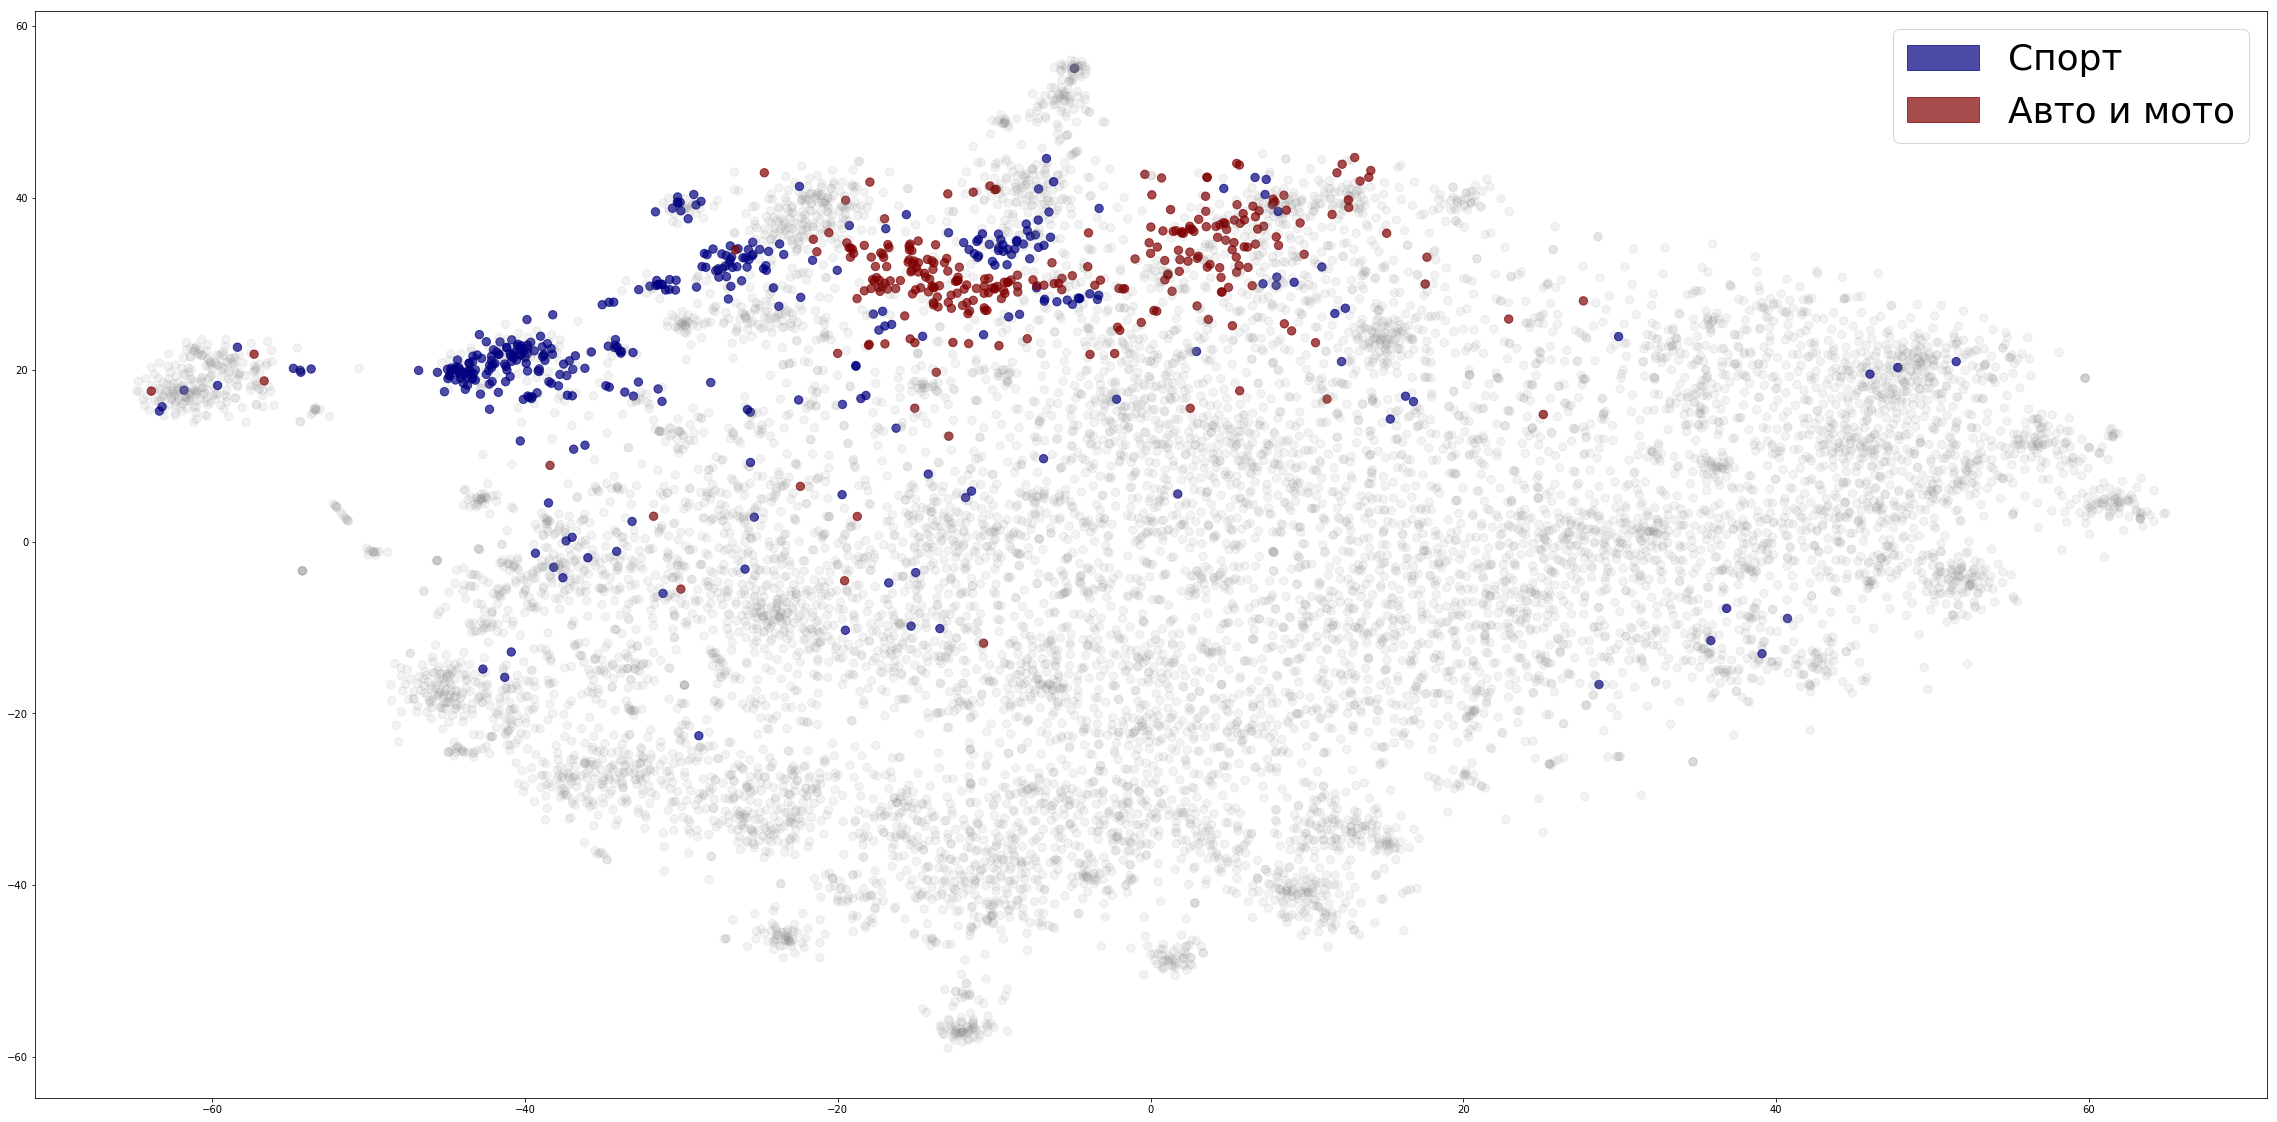
\includegraphics[width=1\textwidth]{index0}
\label{pic:categories}
\end{figure}

Полученное изображение наглядно показывает, что обученная модель действительно получает семантически похожие векторы. Так, сообщества с одинаковыми категориями находятся рядом друг с другом. Интересно, что различные сообщества, интересующие мужскую аудиторию социальной сети, находятся достаточно близко друг к другу. Кроме того, на рисунке можно заметить несколько небольших скоплений сообщества с категорией <<Спорт>>, относящиеся к разным видам спорта.  

Дополнительно был обучен алгоритм кластеризации k-means на результирующих многомерных векторах. Было проведено разбиение на 32 кластера, мною была проведена ручная разметка нескольких из них. (см. рис. \ref{pic:clusters})

\begin{figure}[h]
\caption{Визуализация векторного пространства}
\centering
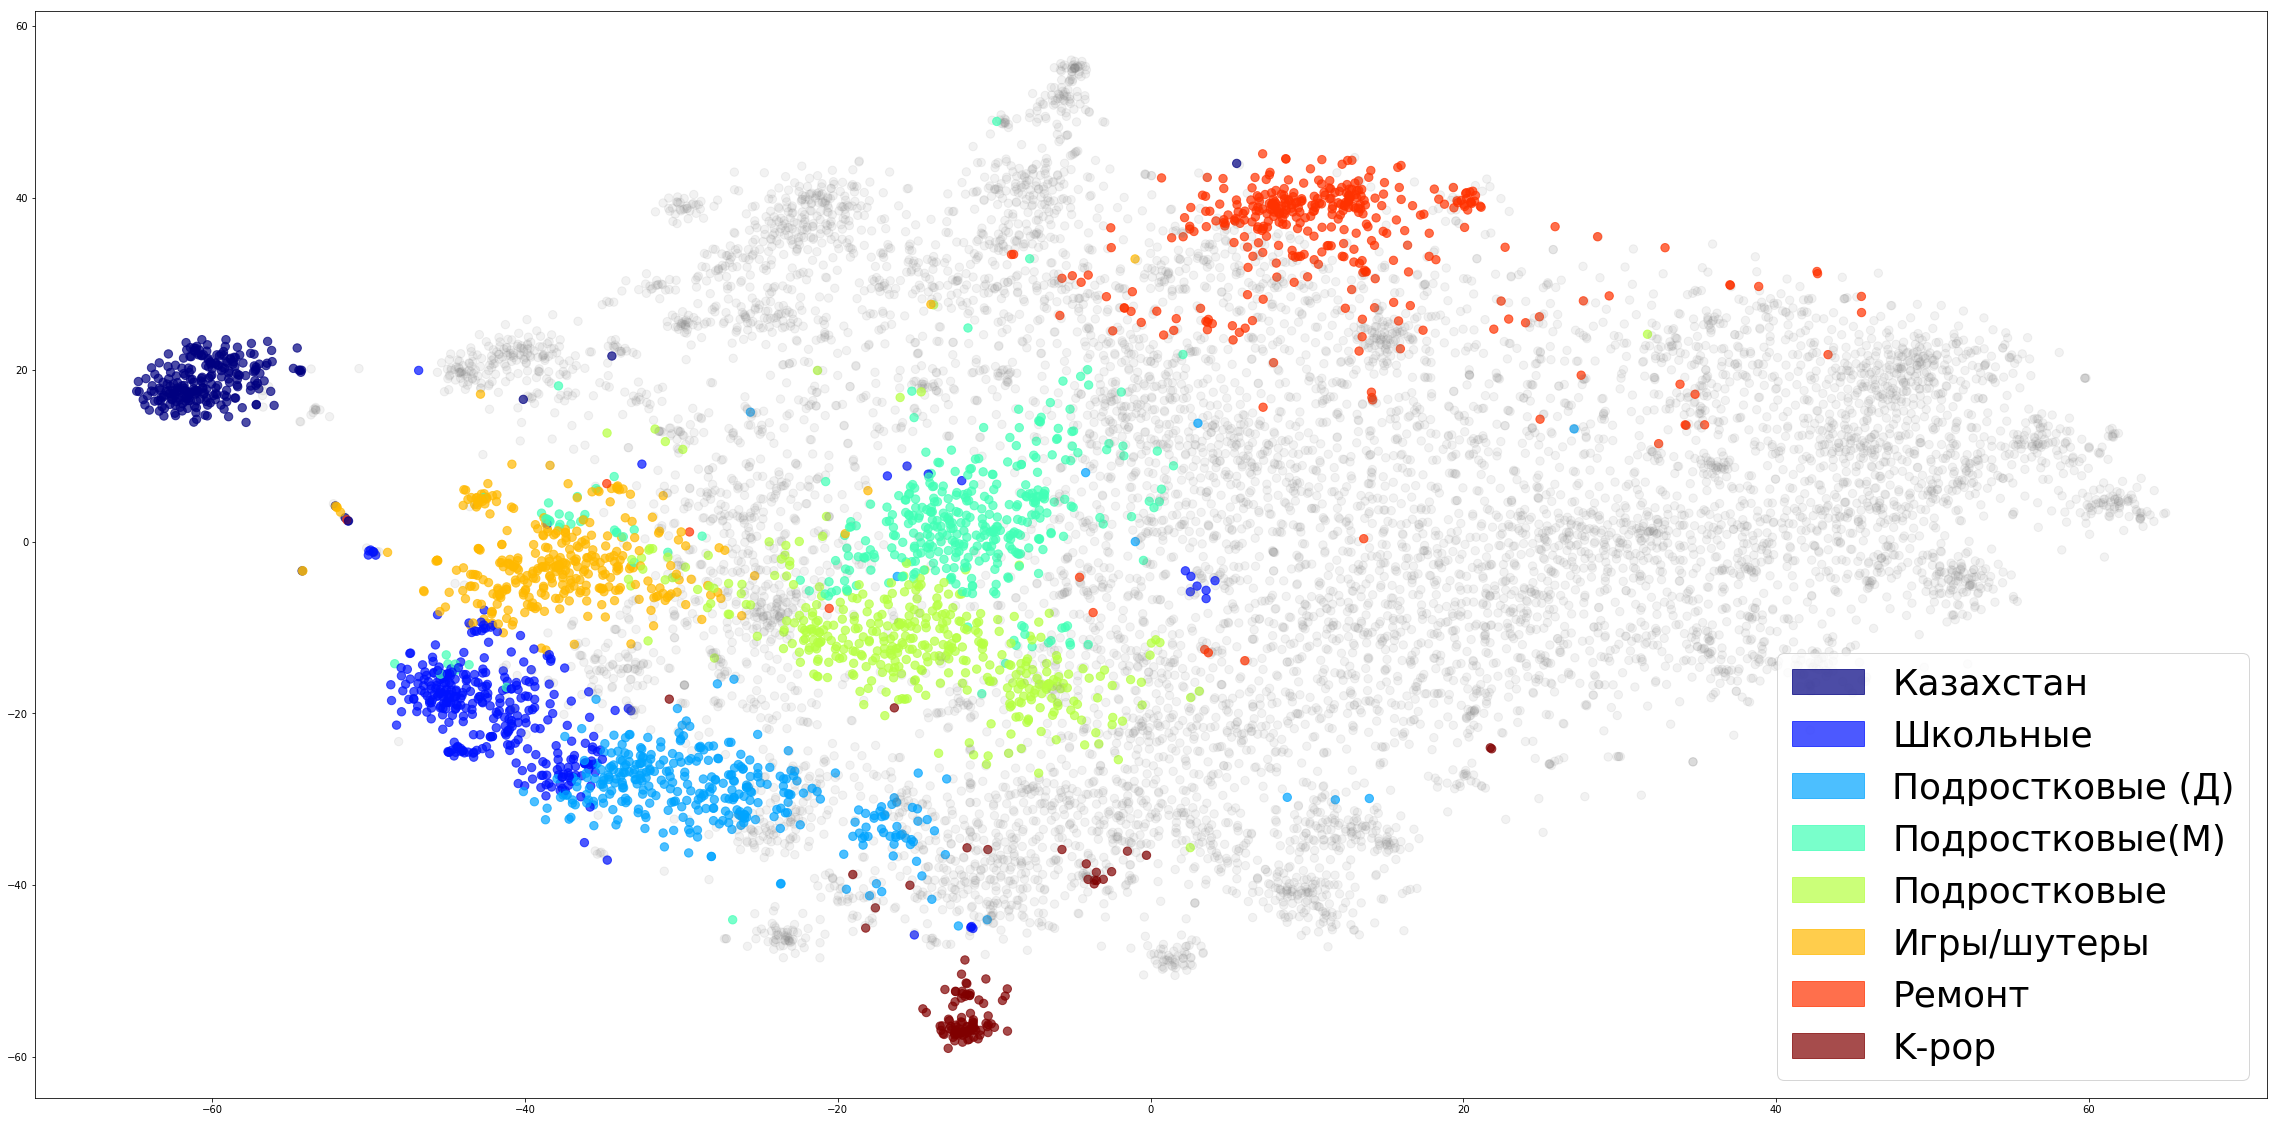
\includegraphics[width=1\textwidth]{clusters}
\label{pic:clusters}
\end{figure}

На рисунке видно, что модель сохраняет важные свойства сообществ. К примеру, в социальной сети существует большое число пользователей из Казахстана, которые создают сообщества, записи в которых ведутся на казахском языке. Заметим, что кластер таких сообществ заметно удалeн от общей картины. 

Возрастные категории пользователей сообществ также учитываются, сообщества тематик, интересующих пользователей школьного возраста расположены рядом с сообществами подростковых тематик, а так же рядом с кластером компьютерных игр. Интересно, что сообщества, которые интересуют юношей, находятся в некотором отдалении от сообществ, привлекающих аудиторию девушек. В то же время оба кластера находятся в близости к кластеру школьных тематик.

Отдельно стоит отметить кластер специфических, но популярных, интересов пользователей, которым является кластер с корейской поп-музыкой (K-pop). Кластер таких сообществ стоит в некотором отдалении от всех остальных, и достаточно близко к сообществам для молодых девушек. Интересно, что согласно интернет-опросам, основная демография слушателей корейской музыки --- молодые девушки. \footnote{https://www.kpopmap.com/age-and-gender-demographics-of-kpop-girl-group-listeners-in-south-korea-2018/}

Сообщества, относящиеся к ремонту, лежат на карте близко с сообществам спортивной и авто тематик (см. рис. \ref{pic:categories}), показывая популярность таких сообществ у мужской части пользователей социальной сети.    

\chapterconclusion

Эксперименты показали, что полученные вектора действительно отвечают главному требованию --- они сохраняют семантический смысл сущностей (сообщества социальной сети). Было показано, что предлагаемая модель работает лучше, чем альтернативные варианты. Дополнительным преимуществом модели является меньшая требовательность к ресурсам оборудования, на котором она обучается. 

Использование полученных векторов в моделях машинного обучения для решения спектра различных задач показало, что полученные векторы могут быть применены на практике в других алгоритмах. Кроме того, гибкость моделей и возможность работать с различными типами данных позволяет использовать конкретную модель получения векторов, подстраиваясь под условия задачи. Эксперимент показал, что различные вариации модели позволяют лучше решать задачи, в зависимости от их контекста. 


%% Макрос для заключения. Совместим со старым стилевиком.
\startconclusionpage

В данной работе былм предложены модели выделения векторного представления сообществ на основе сессионных действий пользователя. Было предложено 3 вариации конечной модели, для работы с подписками и отписками пользователей (п. \ref{sec:algo-subs}), лайками пользователей (п. \ref{sec:algo-likes}) и комбинированный подход, учитывающий оба типа событий (п. \ref{sec:algo-combined})

Экспериментально было показано, что векторы, полученные в результате обучения моделей, могут быть применены для решения других задач, таких как классификация сообществ по признакам (категория или геолокация), предсказание следующего действия пользователя (может быть использовано в рекомендательных системах), кластеризация сообществ (может быть использовано для рекламы сообществ).

3 вариации модели показывают гибкость, и, как показывают эксперименты, разные вариации модели могут быть успешно использованы в различных задачах. 

Модель в дальнейшем может быть расширена на более широкий спектр действий пользователей (других слабых событий, таких как клики пользователя на сообщества) 

\printmainbibliography

%% После этой команды chapter будет генерировать приложения, нумерованные русскими буквами.
%% \startappendices из старого стилевика будет делать то же самое
\appendix

\chapter{Результаты классификации категорий сообществ}\label{app}

\begin{table}[!h]
\caption{Классификация общих категорий (данные по подпискам)}\label{tab-subs-g}
\centering
\begin{tabular}{|*{18}{c|}}\hline
Категория & \thead{Предложенная \\  модель}  & Raw data & ALS & LDA \\\hline
Спорт        							& 0.667 $\pm$ 0.043 & 0.209 $\pm$ 0.054 & 0.481 $\pm$ 0.041 & 0.553 $\pm$ 0.090 \\\hline
\thead{Городское \\ сообщество}
                                      		& 0.231 $\pm$ 0.036 & 0.085 $\pm$ 0.018 & 0.111 $\pm$ 0.022 & 0.336 $\pm$ 0.023  \\\hline
Музыка         				    	& 0.296 $\pm$ 0.041 & 0.131 $\pm$ 0.030 & 0.082 $\pm$ 0.023 & 0.022 $\pm$ 0.014  \\\hline
\thead{Сообщество \\ по интересам}
         									& 0.078 $\pm$ 0.026 & 0.153 $\pm$ 0.017 & 0.054 $\pm$ 0.011 & 0.119 $\pm$ 0.033  \\\hline
Образование              		& 0.319 $\pm$ 0.033 & 0.136 $\pm$ 0.031 & 0.263 $\pm$ 0.028 & 0.232 $\pm$ 0.026  \\\hline
Семья  								& 0.322 $\pm$ 0.027 & 0.147 $\pm$ 0.020 & 0.043 $\pm$ 0.015 & 0.184 $\pm$ 0.041  \\\hline
\thead{Известная \\ личность}
         							    	& 0.315 $\pm$ 0.025 & 0.139 $\pm$ 0.025 & 0.182 $\pm$ 0.037 & 0.185 $\pm$ 0.032   \\\hline
\thead{Здоровье \\ и красота}
               							    & 0.522 $\pm$ 0.019 & 0.232 $\pm$ 0.028 & 0.309 $\pm$ 0.046 & 0.374 $\pm$ 0.028  \\\hline
\thead{Культурное \\ общество}
           									& 0.400 $\pm$ 0.018 & 0.282 $\pm$ 0.010 & 0.339 $\pm$ 0.014 & 0.380 $\pm$ 0.017  \\\hline
Развлечения           			& 0.616 $\pm$ 0.017 & 0.492 $\pm$ 0.015 & 0.590 $\pm$ 0.010 & 0.578 $\pm$ 0.013  \\\hline
\textbf{Средн. взвеш.}& \textbf{0.452 $\pm$ 0.012} & 0.301 $\pm$ 0.009 & 0.356 $\pm$ 0.010 & 0.391 $\pm$ 0.014  \\\hline
\end{tabular}
\end{table}


\begin{table}[!h]
\caption{Классификация подробных категорий (данные по подпискам)}\label{tab-subs-d}
\centering
\begin{tabular}{|*{18}{c|}}\hline
Категория & \thead{Предложенная \\  модель}  & Raw data & ALS & LDA  \\\hline
\thead{Отношения  \\ полов}                   
											 & 0.284 $\pm$ 0.043 & 0.116 $\pm$ 0.015 & 0.106 $\pm$ 0.056 & 0.222 $\pm$ 0.041 \\\hline
\thead{Молодежная \\ организация}   
											 & 0.410 $\pm$ 0.068 & 0.155 $\pm$ 0.037 & 0.336 $\pm$ 0.030 & 0.323 $\pm$ 0.054  \\\hline
\thead{Рецепты \\ и еда}        
											 & 0.782 $\pm$ 0.030 & 0.306 $\pm$ 0.056 & 0.628 $\pm$ 0.027 & 0.685 $\pm$ 0.052 \\\hline
\thead{Городское \\ сообщество}                        
											 & 0.540 $\pm$ 0.022 & 0.110 $\pm$ 0.015 & 0.249 $\pm$ 0.016 & 0.500 $\pm$ 0.026 \\\hline
Кино                      				 & 0.577 $\pm$ 0.050 & 0.195 $\pm$ 0.024 & 0.463 $\pm$ 0.026 & 0.349 $\pm$ 0.049 \\\hline
Фотография                      & 0.352 $\pm$ 0.016 & 0.137 $\pm$ 0.022 & 0.327 $\pm$ 0.040 & 0.301 $\pm$ 0.017 \\\hline
Образование                     & 0.566 $\pm$ 0.018 & 0.194 $\pm$ 0.025 & 0.434 $\pm$ 0.041 & 0.388 $\pm$ 0.012 \\\hline
Литература                       & 0.463 $\pm$ 0.039 & 0.157 $\pm$ 0.030 & 0.416 $\pm$ 0.028 & 0.333 $\pm$ 0.026 \\\hline
Творчество                        & 0.292 $\pm$ 0.022 & 0.190 $\pm$ 0.039 & 0.170 $\pm$ 0.029 & 0.298 $\pm$ 0.033 \\\hline
Юмор                                  & 0.716 $\pm$ 0.017 & 0.458 $\pm$ 0.012 & 0.659 $\pm$ 0.028 & 0.644 $\pm$ 0.017 \\\hline
\textbf{Средн. взвеш.} & \textbf{0.548 $\pm$ 0.010} & 0.266 $\pm$ 0.010 & 0.453 $\pm$ 0.014 & 0.456 $\pm$ 0.007 \\\hline
\end{tabular}
\end{table}

% ------------------

\begin{table}[!h]
\caption{Классификация общих категорий (данные по лайкам)}\label{tab-likes-g}
\centering
\begin{tabular}{|*{18}{c|}}\hline
Категория & \thead{Предложенная \\  модель}  & Raw data & ALS & LDA \\\hline
Музыка         				    	& 0.152 $\pm$ 0.039 & 0.062 $\pm$ 0.015 & 0.005 $\pm$ 0.011 & 0.020 $\pm$ 0.010  \\\hline
\thead{Известная \\ личность}
         							    	& 0.093 $\pm$ 0.050 & 0.042 $\pm$ 0.014 & 0.047 $\pm$ 0.048 & 0.088 $\pm$ 0.025 \\\hline
Образование              		& 0.055 $\pm$ 0.019 & 0.032 $\pm$ 0.029 & 0.010 $\pm$ 0.013 & 0.044 $\pm$ 0.020 \\\hline
\thead{Городское \\ сообщество}
                                      		& 0.225 $\pm$ 0.035 & 0.099 $\pm$ 0.025 & 0.089 $\pm$ 0.042 & 0.066 $\pm$ 0.033 \\\hline
Спорт        							& 0.612 $\pm$ 0.026 & 0.153 $\pm$ 0.029 & 0.226 $\pm$ 0.034 & 0.488 $\pm$ 0.028 \\\hline
\thead{Сообщество \\ по интересам}
         									& 0.221 $\pm$ 0.021 & 0.074 $\pm$ 0.022 & 0.044 $\pm$ 0.017 & 0.163 $\pm$ 0.033 \\\hline
\thead{Здоровье \\ и красота}
               							    & 0.411 $\pm$ 0.022 & 0.055 $\pm$ 0.007 & 0.098 $\pm$ 0.017 & 0.172 $\pm$ 0.033 \\\hline
Семья  								& 0.373 $\pm$ 0.044 & 0.045 $\pm$ 0.020 & 0.092 $\pm$ 0.036 & 0.186 $\pm$ 0.010 \\\hline
\thead{Культурное \\ общество}
           									& 0.439 $\pm$ 0.006 & 0.085 $\pm$ 0.016 & 0.282 $\pm$ 0.025 & 0.348 $\pm$ 0.029 \\\hline
Развлечения           			& 0.648 $\pm$ 0.011 & 0.530 $\pm$ 0.009 & 0.565 $\pm$ 0.009 & 0.575 $\pm$ 0.009 \\\hline
\textbf{Средн. взвеш.}& \textbf{0.459 $\pm$ 0.007} & 0.242 $\pm$ 0.010 & 0.307 $\pm$ 0.008 & 0.358 $\pm$ 0.013 \\\hline
\end{tabular}
\end{table}

\begin{table}[!h]
\caption{Классификация подробных категорий (данные по лайкам)}\label{tab-likes-d}
\centering
\begin{tabular}{|*{18}{c|}}\hline
Категория & \thead{Предложенная \\  модель}  & Raw data & ALS & LDA  \\\hline
\thead{Отношения  \\ полов}                   
											 & 0.382 $\pm$ 0.047 & 0.114 $\pm$ 0.037 & 0.115 $\pm$ 0.059 & 0.150 $\pm$ 0.009  \\\hline
\thead{Рецепты \\ и еда}        
											 & 0.796 $\pm$ 0.016 & 0.163 $\pm$ 0.027 & 0.401 $\pm$ 0.056 & 0.438 $\pm$ 0.069  \\\hline
\thead{Молодежная \\ организация}   
											 & 0.540 $\pm$ 0.064 & 0.088 $\pm$ 0.021 & 0.120 $\pm$ 0.023 & 0.286 $\pm$ 0.045  \\\hline
Кино                      				 & 0.618 $\pm$ 0.014 & 0.133 $\pm$ 0.030 & 0.072 $\pm$ 0.029 & 0.226 $\pm$ 0.032  \\\hline
\thead{Городское \\ сообщество}                        
											 & 0.479 $\pm$ 0.045 & 0.109 $\pm$ 0.018 & 0.337 $\pm$ 0.034 & 0.202 $\pm$ 0.043  \\\hline
Образование                     & 0.303 $\pm$ 0.034 & 0.078 $\pm$ 0.021 & 0.054 $\pm$ 0.024 & 0.115 $\pm$ 0.031  \\\hline
Фотография                      & 0.444 $\pm$ 0.029 & 0.067 $\pm$ 0.018 & 0.054 $\pm$ 0.027 & 0.217 $\pm$ 0.038  \\\hline
Творчество                        & 0.393 $\pm$ 0.038 & 0.113 $\pm$ 0.041 & 0.146 $\pm$ 0.014 & 0.227 $\pm$ 0.040  \\\hline
Литература                       & 0.467 $\pm$ 0.022 & 0.161 $\pm$ 0.039 & 0.195 $\pm$ 0.029 & 0.324 $\pm$ 0.024  \\\hline
Юмор                                  & 0.749 $\pm$ 0.012 & 0.482 $\pm$ 0.020 & 0.596 $\pm$ 0.014 & 0.595 $\pm$ 0.016  \\\hline
\textbf{Средн. взвеш.} & \textbf{0.575 $\pm$ 0.013} & 0.247 $\pm$ 0.014 & 0.322 $\pm$ 0.007 & 0.370 $\pm$ 0.016  \\\hline
\end{tabular}
\end{table}

% ------------------

\begin{table}[!h]
\caption{Классификация общих категорий (комбинированные данные)}\label{tab-combined-g}
\centering
\begin{tabular}{|*{18}{c|}}\hline
Категория & \thead{Предложенная \\  модель}  & Raw data & ALS & LDA \\\hline
Музыка         				    	& 0.340 $\pm$ 0.046 & 0.066 $\pm$ 0.018 & 0.075 $\pm$ 0.046 & 0.075 $\pm$ 0.028  \\\hline
\thead{Городское \\ сообщество}
                                      		& 0.269 $\pm$ 0.078 & 0.098 $\pm$ 0.040 & 0.091 $\pm$ 0.030 & 0.455 $\pm$ 0.053  \\\hline
Образование              		& 0.252 $\pm$ 0.054 & 0.121 $\pm$ 0.029 & 0.173 $\pm$ 0.041 & 0.183 $\pm$ 0.034  \\\hline
Спорт        							& 0.726 $\pm$ 0.033 & 0.195 $\pm$ 0.042 & 0.375 $\pm$ 0.048 & 0.601 $\pm$ 0.034  \\\hline
\thead{Известная \\ личность}
         							    	& 0.293 $\pm$ 0.043 & 0.150 $\pm$ 0.025 & 0.154 $\pm$ 0.026 & 0.284 $\pm$ 0.017  \\\hline
\thead{Сообщество \\ по интересам}
         									& 0.123 $\pm$ 0.053 & 0.075 $\pm$ 0.031 & 0.156 $\pm$ 0.014 & 0.242 $\pm$ 0.039  \\\hline
Семья  								& 0.418 $\pm$ 0.030 & 0.168 $\pm$ 0.016 & 0.194 $\pm$ 0.031 & 0.291 $\pm$ 0.026  \\\hline
\thead{Здоровье \\ и красота}
               							    & 0.571 $\pm$ 0.031 & 0.225 $\pm$ 0.027 & 0.295 $\pm$ 0.031 & 0.393 $\pm$ 0.039  \\\hline
\thead{Культурное \\ общество}
           									& 0.468 $\pm$ 0.019 & 0.282 $\pm$ 0.025 & 0.346 $\pm$ 0.013 & 0.397 $\pm$ 0.020  \\\hline
Развлечения           			& 0.673 $\pm$ 0.009 & 0.499 $\pm$ 0.004 & 0.586 $\pm$ 0.010 & 0.621 $\pm$ 0.010  \\\hline
\textbf{Средн. взвеш.}& \textbf{0.511 $\pm$ 0.012} & 0.303 $\pm$ 0.004 & 0.373 $\pm$ 0.012 & 0.449 $\pm$ 0.009  \\\hline
\end{tabular}
\end{table}

\begin{table}[!h]
\caption{Классификация подробных категорий (комбинированные данные)}\label{tab-combined-d}
\centering
\begin{tabular}{|*{18}{c|}}\hline
Категория & \thead{Предложенная \\  модель}  & Raw data & ALS & LDA  \\\hline
\thead{Отношения  \\ полов}                   
											 & 0.298 $\pm$ 0.025 & 0.084 $\pm$ 0.033 & 0.124 $\pm$ 0.045 & 0.247 $\pm$ 0.035  \\\hline
\thead{Молодежная \\ организация}   
											 & 0.477 $\pm$ 0.019 & 0.128 $\pm$ 0.029 & 0.301 $\pm$ 0.034 & 0.412 $\pm$ 0.047  \\\hline
\thead{Городское \\ сообщество}                        
											 & 0.525 $\pm$ 0.014 & 0.074 $\pm$ 0.019 & 0.316 $\pm$ 0.052 & 0.583 $\pm$ 0.026  \\\hline
\thead{Рецепты \\ и еда}        
											 & 0.834 $\pm$ 0.041 & 0.213 $\pm$ 0.040 & 0.646 $\pm$ 0.023 & 0.687 $\pm$ 0.042  \\\hline
Кино                      				 & 0.650 $\pm$ 0.042 & 0.180 $\pm$ 0.027 & 0.362 $\pm$ 0.020 & 0.376 $\pm$ 0.092  \\\hline
Фотография                      & 0.438 $\pm$ 0.029 & 0.141 $\pm$ 0.034 & 0.302 $\pm$ 0.024 & 0.329 $\pm$ 0.036  \\\hline
Образование                     & 0.535 $\pm$ 0.059 & 0.169 $\pm$ 0.021 & 0.332 $\pm$ 0.030 & 0.326 $\pm$ 0.041  \\\hline
Творчество                        & 0.407 $\pm$ 0.058 & 0.147 $\pm$ 0.036 & 0.220 $\pm$ 0.028 & 0.337 $\pm$ 0.050  \\\hline
Литература                       & 0.464 $\pm$ 0.036 & 0.172 $\pm$ 0.023 & 0.476 $\pm$ 0.023 & 0.467 $\pm$ 0.031  \\\hline
Юмор                                  & 0.759 $\pm$ 0.012 & 0.510 $\pm$ 0.016 & 0.664 $\pm$ 0.016 & 0.680 $\pm$ 0.009  \\\hline
\textbf{Средн. взвеш.} & \textbf{0.599 $\pm$ 0.007} & 0.281 $\pm$ 0.009 & 0.460 $\pm$ 0.011 & 0.511 $\pm$ 0.013  \\\hline
\end{tabular}
\end{table}

%\begin{table}[!h]
%\caption{Классификация общих категорий}
%\centering
%\begin{tabular}{|*{18}{c|}}\hline
%Данные & \thead{Предложенная \\ модель}  & Raw data & ALS & LDA  \\\hline
%Подписки            & \textbf{0.562} & 0.374 & 0.512 & 0.510   \\\hline
%Лайки           & \textbf{0.585} & 0.374 & 0.450 & 0.509 \\\hline
%Подписки + лайки           & \textbf{0.578} & 0.388 & 0.531 & 0.557  \\\hline
%\end{tabular}
%\end{table}
%
%\begin{table}[!h]
%\caption{Классификация подробных категорий}
%\centering
%\begin{tabular}{|*{18}{c|}}\hline
%Данные & \thead{Предложенная \\ модель}  & Raw data & ALS & LDA  \\\hline
%Подписки             & \textbf{0.669} & 0.376 & 0.627 & 0.585    \\\hline
%Лайки           &  \textbf{0.641} & 0.427 & 0.483 & 0.543 \\\hline
%Подписки + лайки           & \textbf{0.645} & 0.429 & 0.601 & 0.631  \\\hline
%\end{tabular}
%\end{table}

\end{document}
